\chapter{Deadlock}

\epigraph{No, you can't always get what you want
\\You can't always get what you want
\\You can't always get what you want
\\But if you try sometime you find
\\You get what you need}{The philosphers Jagger \& Richards}

\gls{Deadlock} is defined as when the system cannot make and forward progress. In a lot of systems, Deadlock is just avoided by ignore the entire concept \cite[P.237]{silberschatz2006operating}. Have you heard about turn it on and off again? That is partly because of this. For products where the stakes are low when you deadlock (User Operating Systems, Phones), it may be more efficient not not keep track of all of the allocations in order to keep deadlock from happening. But in the cases where "failure is not an option" - Apollo 13, you need a system that tracks deadlock or better yet prevents it entirely. Take the Apollo 13 module. It may have not failed because of deadlock, but probably wouldn't be good to restart the system on liftoff.

Mission critical operating systems need this guarentee formally because playing the odds with people's lives isn't a good idea. Okay so how do we do this? We model the problem. Even though it is a common statistical phrase that all models are wrong, the more accurate the model is to the system that we are working with the better chance that it'll work better.

\section{Resource Allocation Graphs}

\begin{wrapfigure}[13]{r}{.35\textwidth}
  \begin{center}
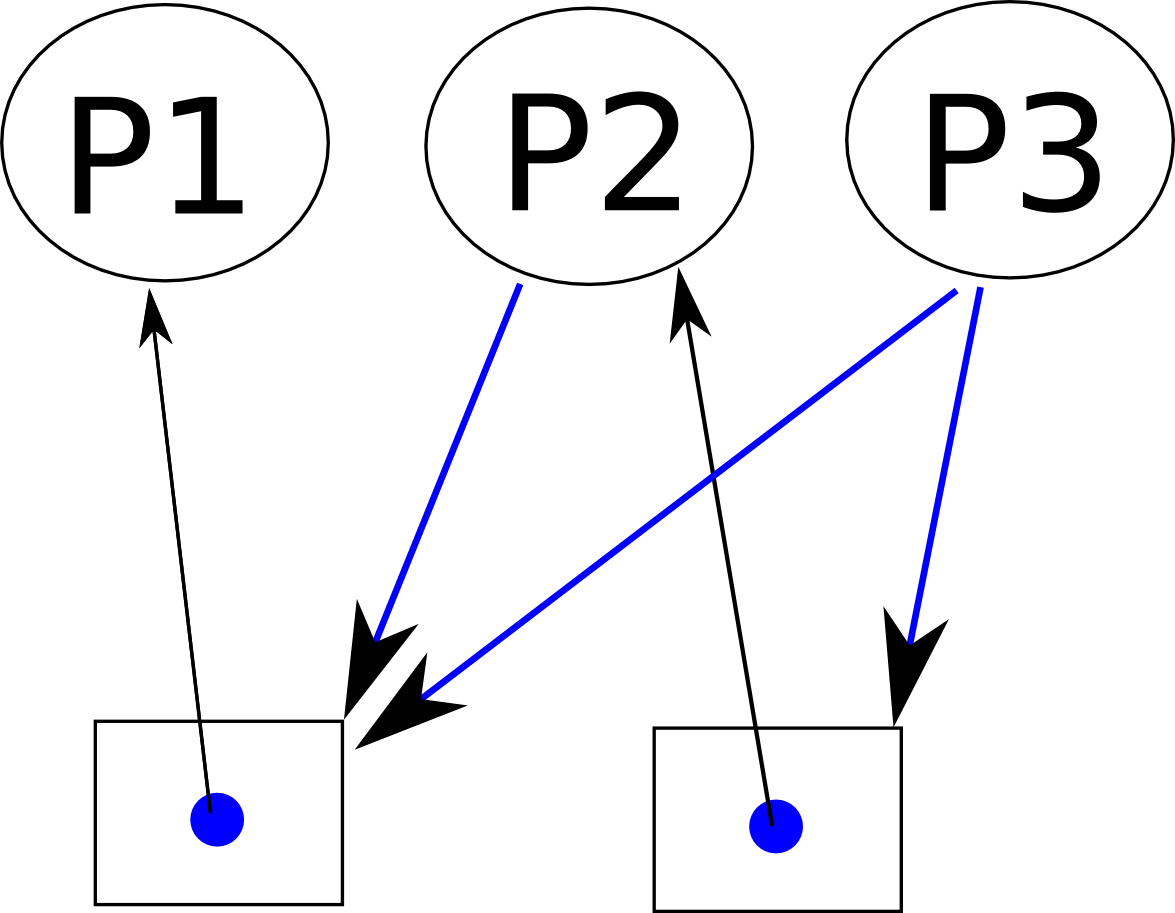
\includegraphics[width=.25\textwidth]{deadlock/images/resource_allocation.png}
\end{center}
  \caption{Resource allocation graph}
\end{wrapfigure}

One such way is modeling the system with a resource allocation graph (\gls{RAG}). A resource allocation graph tracks which resource is held by which process and which process is waiting for a resource of a particular type. It is very powerful and simple tool to illustrate how interacting processes can deadlock. If a process is \emph{using} a resource, an arrow is drawn from the resource node to the process node. If a process is \emph{requesting} a resource, an arrow is drawn from the process node to the resource node.If there is a cycle in the Resource Allocation Graph and each resource in the cycle provides only one instance, then the processes will deadlock. For example, if process 1 holds resource A, process 2 holds resource B and process 1 is waiting for B and process 2 is waiting for A, then process 1 and 2 process will be deadlocked.

\begin{wrapfigure}[12]{r}{.35\textwidth}
  \begin{center}
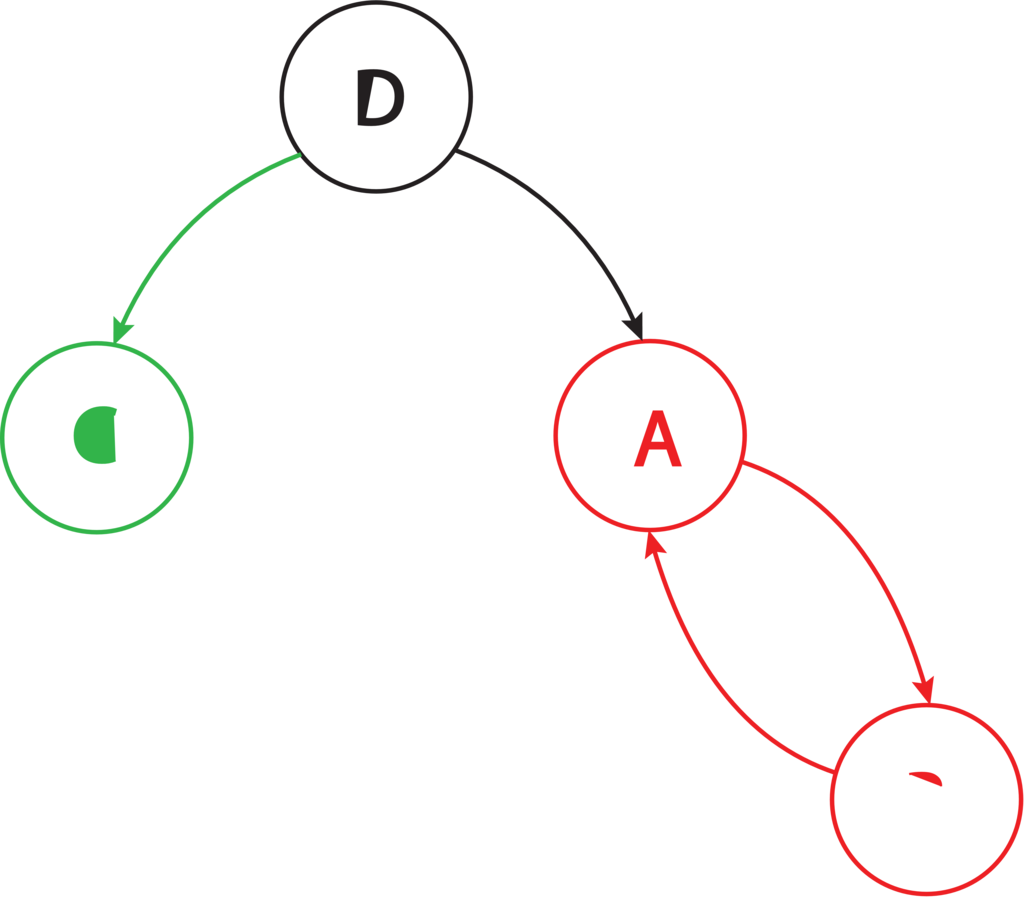
\includegraphics[width=.25\textwidth]{deadlock/images/colorful.png}
\end{center}
  \caption{Colorful Deadlock}
\end{wrapfigure}

Consider the following resource allocation graph. Assume that the processes ask for exclusive access to the file. If you have a bunch of processes running and they request resources and the operating system ends up in this state, you deadlock! You may not see this because the operating system may \textbf{preempt} some processes breaking the cycle but there is still a change that your three lonely processes could deadlock. You can also make these kind of graphs with \texttt{make} and rule dependencies with our parmake MP for example.

\section{Coffman conditions}

There are four \emph{necessary} and \emph{sufficient} conditions for deadlock -- meaning if these conditions hold then there is a non-zero probability that the system will deadlock at any given iteration. These are known as the \gls{Coffman Conditions} \cite{coffman1971system}.

\begin{itemize}
\tightlist
\item
  \gls{Mutual Exclusion}: no two processes can obtain a resource at the same time.
\item
  \gls{Circular Wait}: there exists a cycle in the Resource Allocation Graph, or there exists a set of processes \{P1,P2,\ldots{}\} such that P1 is waiting for resources held by P2, which is waiting for P3,\ldots{}, which is waiting for P1.
\item
  \gls{Hold and Wait}: a process once obtaining a resource does not let go.
\item
  \gls{No pre-emption}: nothing can force the process to give up a resource.
\end{itemize}

\begin{proof} Deadlock can happen if and only if the four coffman conditions are satisified.

$\rightarrow$ If the system is deadlocked, the four coffman conditions are apparent.

\begin{itemize}
\item For the purposes of contradiction, assume that there is no cicular wait. If not then that means the resource wait graph is acyclic, meaning that there is at least one one process that is not waiting on any resources or it can grab a resource. Since the system can move forward, the system is not deadlocked.
\item For the purposes of contradiction, assume that there is no mutual exclusion. If not, that means that no process is waiting on any other process for a resource. This breaks circular wait and the previous argument proves correctness.
\item For the purposes of contradiction, assume that processes don't hold and wait but our system still deadlocks. Since we have circular wait from the first condition at least one process must be waiting on another process. If that and processes don't hold and wait, that means one process must let go of a resource. Since the system has moved forward, it cannot be deadlocked.
\item For the purposes of contradiction, assume that we have preemption, but the system cannot be un-deadlocked. Have one process, or create one process, that recognizes the circular wait that must be apprent from above and break on the of the links. By the first branch, we must not have deadlock.
\end{itemize}

$\leftarrow$ If the four conditions are apparent, the system is deadlocked. We will prove that if the system is not deadlocked, the four conditions are not apparent. Though this proof is not formal, let us build a system with the three requirements not including circular wait. Let assume that there is a set of processes $P = \{p_1, p_2, ..., p_n\}$ and there is a set of resources $R = \{r_1, r_2, ..., r_m\}$. For simplicity, a process can only request one resource at a time but the proof can be generalized to multiple. Let assume that the system is at different states at different times $t$. Let us assume that the state of the system is a tuple $(h_t, w_t)$ where there are two function $h_t: R \rightarrow P \cup \{\text{unassigned}\}$ that maps resources to the processes that own them (this is a function, meaning that we have mutual exclusion) and or unassigned and $w_t: P \rightarrow R \cup \{\text{satisfied}\}$ that maps the requests that each process makes to a resource or if the process is satisfied. Let $L_t \subseteq P \times R$ be a set of list of requests that a process uses to release a resource at any given time. The evolution of the system is at each step at every time.

\begin{itemize}
\item Release all resources in $L_t$ the a process requests to resource.
\item Find a process that is requesting a resource
\item If that resource is available give it to that process, generating a new $(h_t, w_t)$ and exit the current iteration.
\item Else find another process and try the above if.
\end{itemize}

If all processes have been surveyed and none updates the system, consider it deadlocked. More formally, this system is deadlocked means  if $\exists t_0, \forall t \geq t_0, \forall p \in P, w_t(p) \neq \text{satisfied} \text{ and } \exists q, q \neq p \rightarrow h_t(w_t(p)) = q$ (which is what we need to prove). 
\begin{proof} These conditions imply deadlock. 
Deadlock for a system is defined as no work can be done now or later. Work can be done if a process is satisfied, or we can release a resource to a process. No process is satisfied by definition. Since the system can't preempt and release resources (by no preemption), the processes have to do it themselves. If the processes has a resource, it will not let it go until after it is satisfied by hold and wait. All resources requested by the processes are owned by other processes meaning that no process will let any resource go. Since we have shown no processes will give up a resource and no process is satisfied, the system is in deadlock.
\todo{Formalize Subproof}
\end{proof}
The last condition to address is circular wait. Circular wait means that there exists $\forall p \in P, w_t(p) \neq \text{satisfied} \text{ and } \exists q, q \neq p \rightarrow h_t(w_t(p)) = q$. Which is what we needed to show.
\end{proof}

If you break any of them, you cannot have deadlock! Consider the scenario where two students need to write both pen and paper and there is only one of each. Breaking mutual exclusion means that the students share the pen and paper. Breaking circular wait could be that the students agree to grab the pen then the paper. As a proof by contradiction, say that deadlock occurs under the rule and the conditions. Without loss of generality, that means a student would have to be waiting on a pen while holding the paper and the other waiting on a pen and holding the paper. We have contradicted ourselves because one student grabbed the paper without grabbing the pen, so deadlock must not be able to occur. Breaking hold and wait could be that the students try to get the pen and then the paper and if a student fails to grab the paper then they release the pen. This introduces a new problem called \textit{livelock} which will be discussed latter. Breaking preemption means that if the two students are in deadlock the teacher can come in and break up the deadlock by giving one of the students one the held on items or tell both students to put the items down.

\gls{livelock} relates to deadlock but it is not exactly deadlock. Consider the breaking hold and wait solution as above. Though deadlock is avoided, if we pick up the same device (a pen or the paper) again and again in the exact same pattern, neither of us will get any writing done. More generally, livelock happens when the process looks like it is executing but no meaningful work is done. Livelock is generally harder to detect because the processes generally look like they are working to the outside operating system wheras in deadlock the operating system generally knows when two processes are waiting on a system wide resource. Another problem is that there are nessisary conditions for livelock (i.e. deadlock does not occur) but not sufficient conditions -- meaning there is no set of rules where livelock has to occur. You must formally prove in a system by what is known as an invariant. One has to enumerate each of the steps of a system and if each of the steps eventually (after some finite number of steps) leads to forward progress, the system is not livelocked. There are even better systems that prove bounded waits; a system can only be livelocked for at most $n$ cycles which may be important for something like stock exchanges.

\section{Approaches to solving deadlock}

Ignoring deadlock is the most obvious approach that started the chapter out detailing. Quite humorously, the name for this approach is called the \gls{ostrich algorithm}. Though there is no apparent source, the idea for the algorithm comes from the concept of an ostrich sticking its head in the sand. When the operating system detects deadlock, it does nothing out of the ordinary and hopes that the deadlock goes away. Now this is a slight misnomer because the operating system doesn't do anything \textit{abnormal} -- it is not like an operating system deadlocks every few minutes because it runs ~100 processes all requesting shared libraries. An operating system still preempts processes when stopping them for context switches. The operating system has the ability to interrupt any system call, potentially breaking a deadlock scenario. The OS also makes some files read-only thus making the resource shareable. What the algorithm refers to is that if there is an adversary that specifically crafts a program -- or equivalently a user who poorly writes a program -- that deadlock could not be caught by the operating system. For everyday life, this tends to be fine. When it is not we can turn to the following method.

Deadlock detection allows the system to enter a deadlocked state. After entering, the system uses the information that it has to break deadlock. As an example, consider multiple processes accessing files. The operating system is able to keep track of all of the files/resources through file descriptors at some level either abstracted through an API or directly. If the operating system detects a directed cycle in the operating system file descriptor table it may break one process' hold through scheduling for example and let the system proceed. Why this is a popular choice in this realm is that there is no way of knowing which resources a program will select without running the program. This is an extension of Rice's theorem \cite{rice} that says that we cannot know any semantic feature without running the program (semantic meaning like what files it tries to open). So theoretically, it is sound. The problem then gets introduced that we could reach a livelock scenario if we preempt a set of resources again and again. The way around this is mostly probabilistic. The operating system chooses a random resource to break hold and wait. Now even though a user can craft a program where breaking hold and wait on each resource will result in a livelock, this doesn't happen as often on machines that run programs in practice or the livelock that does happen happens for a couple of cycles. These kind of systems are good for products that need to maintain a non-deadlocked state but can tolerate a small chance of livelock for a short period of time. The following proof \textbf{is not required for our 241 related puproses but is included for concreteness}.

\begin{proof} 
That livelock terminates with high probability. This meaning that for any probability level $l$ we can produce a number of iterations $n$ that the probability that the system is not livelocked after that state is at least $l$.

Let $L = \{p_1, p_2, p_3, ...\}$ be an infinite set that has probabilities if we choose a resource that causes livelock in the $i$th iteration of the livelocked by breaking a random resource. Also let the set have the property that $\forall i > 0, \exists j > i, p_j < 1$ Meaning that for all elements after any given element that there is atleast one element int he future that has a probability of breaking deadlock. The probability that the system is not livelocked after $n$ iterations is
\[
P(n) = 1 - \prod\limits_{i = 1}^{n}p_i
\]
Consider the new set $E = \{s_1, s_2, s_3, ...\}$ obtained by selecting all non-one elements. The set must be infinite by our sets property. It is easy to show that 
\[
\prod\limits_{i = 1}^{n}p_i = \prod\limits_{i = 1}^{n}s_i
\]
And since
\[
P(n) = 1 - \prod\limits_{i = 1}^{n}s_i
\]
is a strictly monotonically decreasing function, it must pass the threshold for the probability level at some point. More rigorously
\begin{align*}
Y =& \sup E \\
\prod\limits_{i = 1}^{n}s_i <& Y^n \\
1 - \prod\limits_{i = 1}^{n}s_i >& 1 - Y^n \\
P(n) >& 1 - Y^n \\
P(n) >& l \\
1 - Y^n  >& l \\
\log_Y(1 - l) <& n
\end{align*}
We have found the number of steps in the set $E$ and since our set has the property that gaps between non-one elements is finite, we can reconstruct the number of iterations by picking an $n$ that satifies the $E$ criteria and just adding the finite gaps together, which is what we needed to show.
\end{proof}

Deadlock prevention is making sure that deadlock cannot happen, meaning that you break a Coffman condition. This works the best inside a single program and the software engineer making the choice to break a certain coffman condition. Consider the \href{https://en.wikipedia.org/wiki/Banker's_algorithm}{Banker's Algorithm} \cite{Dijkstra:1965:CSP:1102034}. It is another algorithm for deadlock avoidance. The whole implementation is outside the scope of this class, just know that there are more generalized algorithms for operating systems.

\begin{aside}
The banker algorithm is actually not too complicated. We can start out with the single resource solution. Let's say that I'm a banker. As a banker I have a finite amount of money. As having a finite amount of money, I want to make loans and eventually get my money back. Let's say that we have a set of $n$ people where each of them have a set amount or a limit $a_i$ ($i$ being the $i$th process) that they need to obtain before they can do any work. I keep track in my book how much I've given to each person $l_i$, and I have some amount of principle $p$ at any given time. For people to request money, they do the following. Consider the state of the system $(A=\{a_1, a_2, ...\}, L=\{l_1, l_2, ...\}, p)$. An assumption of this system is that we have $p > \inf a_i$, or we have enough money to satisfy one person. Also, each person will work for a finite period of time and give back our money.

\begin{itemize}
\item A person $j$ requests $m$ from me
\begin{itemize}
\item if $m < p$, they are denied.
\item if $m + l_j > a_i$ they are denied
\item Pretend we are in a new state $(A=\{..., a_j, ...\}, L=\{.., l_j + m, ...\}, p - m)$ where the process is granted the resource.
\end{itemize}
\item if now person $j$ is either satisfied ($l_j == a_j$) or $\exists i, a_j - l_j < p$. In other words we have enough money to satisfy one other person. If either, consider the transaction safe and give them the money.
\end{itemize}

Why does this work? Well at the start we are in a safe state -- defined by we have enough money to satisfy at least one person. Each of these "loans" results in a safe state. If we have exhausted our reserve, one person is working and will give us money greater than or equal to our previous "loan", thus putting us in a safe state again. Since we always have the ability to make one additional move the system can never deadlock. Now, there is no guarentee that the system won't livelock. If the process we hope to request something never does, no work will be done -- but not due to deadlock. This analogy expands to higher orders of magnitude but requires that either a process can do its work entirely or there exists a process whose combination of resources can be satisfied, which makes the algorithm a little more tricky (an additional for loop) but nothing too bad. There are a fair bit of downsides to this

\begin{itemize}
\item The program first needs to know how much of each resource a process needs. A lot of times that is impossible or the process requests the wrong amount because the programmer didn't forsee it. 
\item The system could livelock. 
\item We know in most systems that resources are generally not homogenous. Of course there are things like pipes and sockets but for the most part there is only 1 of a particular file. This could mean that the runtime of the algorithm could be slow for systems with millions of resources.
\item Also, this can't keep track of resources that come and go. A process may delete a resource as a side effect or create a resource. The algorithm assumes a static allocation and that each process performs a non-destructive operation.
\end{itemize}
\end{aside}

\section{Dining Philosophers}

The Dining Philosophers problem is a classic synchronization problem. Imagine I invite $n$ (let's say 5) philosophers to a meal. We will sit them at a table with 5 chopsticks, one between each philosopher. A philosopher alternates between wanting to eat or think. To eat the philosopher must pick up the two chopsticks either side of their position. The original problem required each philosopher to have two forks, but one can eat with a single fork so we rule this out. However these chopsticks are shared with his neighbor.

\begin{wrapfigure}[10]{r}{.3\textwidth}
  \begin{center}
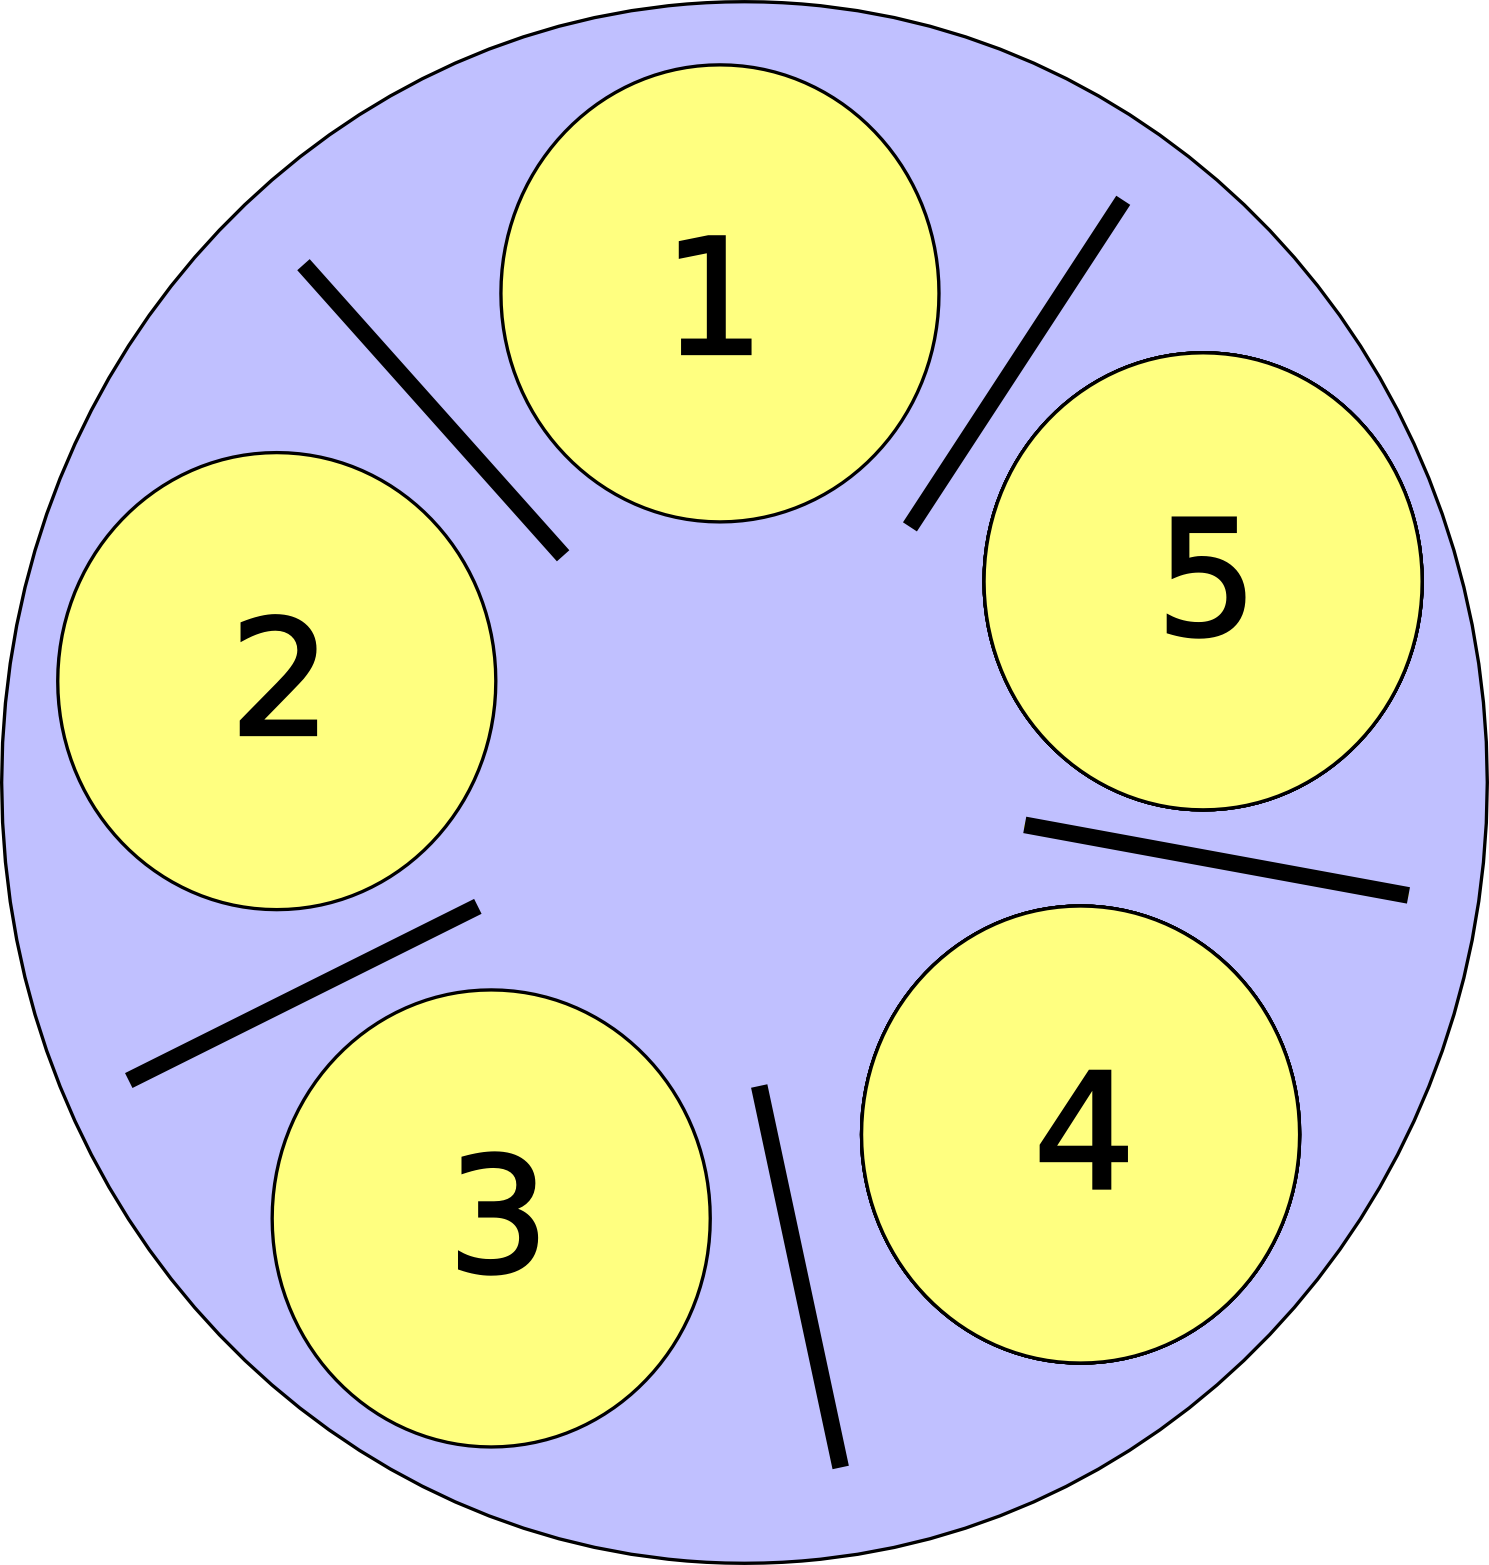
\includegraphics[width=.2\textwidth]{deadlock/images/5DiningPhilosophers.png}
\end{center}
  \caption{Dining Philosophers}
\end{wrapfigure}

Is it possible to design an efficient solution such that all philosophers get to eat? Or, will some philosophers starve, never obtaining a second chopstick? Or will all of them deadlock? For example, imagine each guest picks up the chopstick on their left and then waits for the chopstick on their right to be free. Oops - our philosophers have deadlocked! Each of the philosophers are essentially the same, meaning that each philosopher has the same instruction set based on the other philosopher ie you can't tell every even philosopher to do one thing and every odd philosopher to do another thing.

\subsection{Failed Solutions}

\begin{code}[language=C]
void* philosopher(void* forks){
     info phil_info = forks;
     pthread_mutex_t* left_fork = phil_info->left_fork;
     pthread_mutex_t* right_fork = phil_info->right_fork;
     while(phil_info->simulation){
          pthread_mutex_lock(left_fork);
          pthread_mutex_lock(right_fork);
          eat(left_fork, right_fork);
          pthread_mutex_unlock(left_fork);
          pthread_mutex_unlock(right_fork);
     }
}
\end{code}

This looks good but. What if everyone picks up their left fork and is waiting on their right fork? We have deadlocked the program. It is important to note that deadlock doesn't happen all the time and the probability that this solution deadlocks goes down as the number of philosophers goes up. What is really important to note is that eventually that this solution will deadlock, letting threads starve which is bad. So now you are thinking about breaking one of the coffman conditions. Let's break Hold and Wait!

\begin{code}[language=C]
void* philosopher(void* forks){
     info phil_info = forks;
     pthread_mutex_t* left_fork = phil_info->left_fork;
     pthread_mutex_t* right_fork = phil_info->right_fork;
     while(phil_info->simulation){
          pthread_mutex_lock(left_fork);
          pthread_mutex_lock(right_fork);
          eat(left_fork, right_fork);
          pthread_mutex_unlock(left_fork);
          pthread_mutex_unlock(right_fork);
     }
}
\end{code}

Now our philosopher picks up the left fork and tries to grab the right. If it's available, they eat. If it's not available, they put the left fork down and try again. No deadlock! But, there is a problem. What if all the philosophers pick up their left at the same time, try to grab their right, put their left down, pick up their left, try to grab their right\ldots{}. We have now livelocked our solution! Our poor philosopher are still starving, so let's give them some proper solutions.

\section{Viable Solutions}

The naive arbitrator solution is have one arbitrator (a mutex for example). Have each of the philosopher ask the arbitrator for permission to eat (i.e. trylock the mutex). This solution allows one philosopher to eat at a time. When they are done, another philosopher can ask for permission to eat. This prevents deadlock because there is no circular wait! No philosopher has to wait on any other philosopher. The advanced arbitrator solution is to implement a class that determines if the philosopher's forks are in the arbitrator's possession. If they are, they give them to the philosopher, let him eat, and take the forks back. This has the added bonus of being able to have multiple philosopher eat at the same time.

There are a lot of problems with these solutions. One is that they are slow and have a single point of failure or the arbitrator. Assuming that all the philosophers are good-willed, the arbitrator needs to be fair and be able to determine if a transaction would cause deadlock in the multi-arbitrator case. Further more in practical systems, the arbitrator tends to give forks to the same processes because of scheduling or pseudorandomness. Another important thing to note is that this prevents deadlock for the entire system. But in our model of dining philosophers, the philosopher has to release the lock themselves. Then you can consider the case of the malicious philosopher (let's say Decartes because of his Evil Demons) could hold on to the arbitrator forever. He would make forward progress and the system would make forward progress but there is no way of ensuring that each process makes forward progress without assuming something about the processes or having true preemption -- meaning that a higher authority (let's say Steve Jobs) tells them to stop eating forcibly.

\todo{Prove arbitrator's doesn't deadlock}

\subsection{Leaving the Table (Stallings' Solution)}

Why does the first solution deadlock? Well there are $n$ philosophers and $n$ chopsticks. What if there is only 1 philsopher at the table? Can we deadlock? No. How about 2 philsophers? 3? \ldots{} You can see where this is going. Stallings' \cite[P. 280]{stalling} solutions says to remove philosophers from the table until deadlock is not possible -- think about what the magic number of philosophers at the table. The way to do this in actual system is through semaphores and letting a certain number of philosopher through. This has the benefit that multiple philosophers can be eating.

In the case that the philosophers aren't evil, this solution requires a lot of time-consuming context switching. There is also no reliable way to know the number of resources before hand. In the dining philosophers case, this is solved because everything is known but trying to specify and operating system where you don't know which file is going to get opened by what process leads you with a faulty solution. And again since semaphores are system constructs, they obey system timing clocks which means that the same processes tend to get added back into the queue again. Now if a philosopher becomes evil, then the problem becomes that there is no preemption. A philosopher can eat for as long as they want and the system will continue to function but that means the fairness of this solution can be low in the worst case. This works best with timeouts (or forced context switches) in order to ensure bounded wait times.

\begin{proof} Stallings' Solution Doesn't Deadlock.

Let's number the philosophers $\{p_0, p_1, .., p_{n-1}\}$ and the resources $\{r_0, r_1, .., r_{n-1}\}$. A philosopher $p_i$ needs resource $r_{i-1 \mod n}$ and $r_{i + 1 \mod n}$. Without loss of generality, let us take $p_i$ out of the picture. Each resource had exactly two philosophers that could use it. Now resources $r_{i-1 \mod n}$ and $r_{i + 1 \mod n}$ only have on philosopher waiting on it. Even if hold and wait, no preemption, and mutual exclusion or present, the resources can never enter a state where one philosopher requests them and they are held by another philosopher because only one philosopher can request them. Since there is no way to generate a cycle otherwise, circular wait cannot hold. Since circular wait cannot hold, deadlock cannot happen.

\end{proof}


\subsection{Partial Ordering (Dijkstra's Solution)}

This is Dijkstra's solution \cite[P. 20]{EWD:EWD310}. He was the one to propose this problem on an exam. Why does the first solution deadlock? Dijkstra thought that the last philosopher who picks up his left fork (causing the solution to deadlock) should pick up his right. He accomplishes it by number the forks $1..n$, and tells each of the philosopher to pick up his lower number fork. Let's run through the deadlock condition again. Everyone tries to pick up their lower number fork first. Philosopher $1$ gets fork $1$, Philosopher $2$ gets fork $2$, and so on until we get to Philosopher $n$. They have to choose between fork $1$ and $n$. fork $1$ is already held up by philosopher $1$, so they can't pick up that fork, meaning he won't pick up fork $n$. We have broken circular wait! Meaning deadlock isn't possible.

The problems to this is that an entity either needs to know the finite set of resources or be able to produce a consistent partial order suck that circular wait cannot happen. This also implies that there needs to be some entity, either the operating system or another process, deciding on the number and all of the philosophers need to agree on the number as new resources come in. As we have also see with previous solutions, this relies on context switching so this prioritizes philosophers that have already eaten but can be made more fair by introducing random sleeps and waits.

\todo{Prove dijkstra's doesn't deadlock}


\subsection{Advanced Solutions}

There are many more advanced solutions a non-exhaustive list includes 
\begin{itemize}
\item Clean/Dirty Forks (Chandra/Misra Solution) 
\todo{Detail the Clean/Dirty Solution, and cite}
\item Actor Model (other Message passing models)
\todo{Detail the Actor Model, and cite}
\end{itemize}

\section{Topics}

\begin{itemize}
  \item Coffman Conditions
  \item Resource Allocation Graphs
  \item Dining Philosophers
  \item Failed DP Solutions 
  \item Livelocking DP Solutions 
  \item Working DP Solutions: Benefits/Drawbacks
\end{itemize}

\section{Questions}

\begin{itemize}
\item
  What are the Coffman Conditions?
\item
  What do each of the Coffman conditions mean? (e.g.~can you provide a definition of each one)
\item
  Give a real life example of breaking each Coffman condition in turn. A situation to consider: Painters, Paint, Paintbrushes etc. How would you assure that work would get done?
\item
  Be able to identify when Dining Philosophers code causes a deadlock (or not). For example, if you saw the following code snippet which Coffman condition is not satisfied?

\begin{code}[language=C]
// Get both locks or none
pthread_mutex_lock(a);
if(pthread_mutex_trylock( b )) { /* failure */
  pthread_mutex_unlock( a );
}
\end{code}
\item
  The following calls are made

\begin{code}[language=c]
// Thread 1
pthread_mutex_lock(m1) // success
pthread_mutex_lock(m2) // blocks

// Thread 2
pthread_mutex_lock(m2) // success
pthread_mutex_lock(m1) // blocks
\end{code}

  What happens and why? What happens if a third thread calls
  \texttt{pthread\_mutex\_lock(m1)} ?
\item
  How many processes are blocked? As usual assume that a process is able
  to complete if it is able to acquire all of the resources listed
  below.

  \begin{itemize}
  \tightlist
  \item
    P1 acquires R1
  \item
    P2 acquires R2
  \item
    P1 acquires R3
  \item
    P2 waits for R3
  \item
    P3 acquires R5
  \item
    P1 waits for R4
  \item
    P3 waits for R1
  \item
    P4 waits for R5
  \item
    P5 waits for R1
  \end{itemize}
\end{itemize}

(Draw out the resource graph!)

\bibliographystyle{plainnat}
\bibliography{deadlock/deadlock}